\appendix
%En el ap´endice A se incluir´a el enunciado del TP. En el ap´endice B se incluir´an los
%c´odigos fuente de las funciones relevantes desde el punto de vista num´erico. Resultados
%que valga la pena mencionar en el trabajo pero que sean demasiado espec´ıficos para
%aparecer en el cuerpo principal del trabajo podr´an mencionarse en sucesivos ap´endices
%rotulados con las letras mayusculas del alfabeto romano. Por ejemplo: la demostraci´on
%de una propiedad que aplican para optimizar el algoritmo que programaron para resolver
%un problema.

\section{Enunciado}
\label{ap:enunciado}
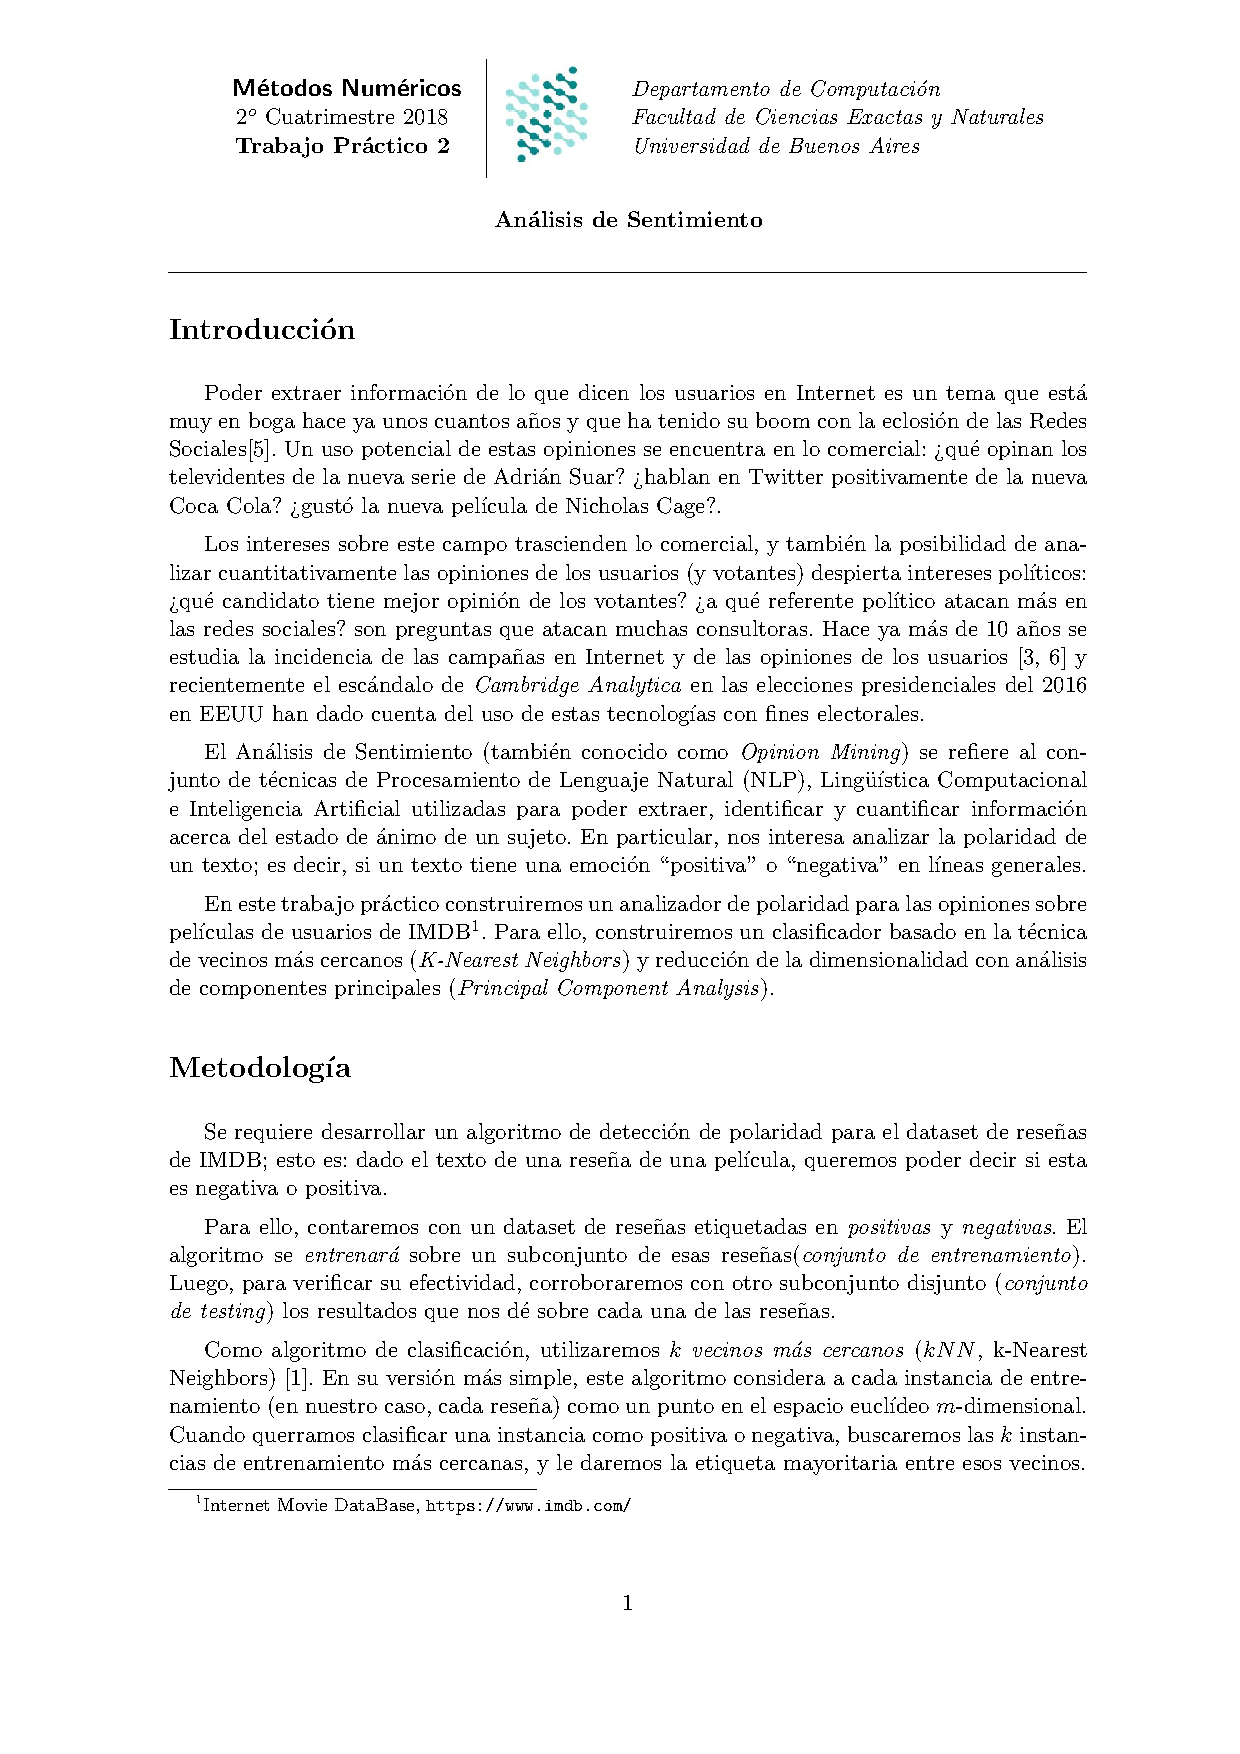
\includepdf[pages=-]{../docs/tp2.pdf}

\section{Código fuente relevante numéricamente}

Código de búsqueda de k vecinos más cercanos (kNN):
\begin{lstlisting}
// Utiliza dist, que simplemente calcula la distancia Manhattan dados dos vectores
bool knn(const VectorizedEntriesMap &entries, const std::vector<double> &words, int k) {
    std::vector<std::pair<double, bool> > distancias;

    for (auto entry:entries) {
        distancias.push_back({
            dist(words, entry.second.bag_of_words),
            entry.second.is_positive});
    }

    MinHeap heapDistancias(distancias.begin(), distancias.end());

    int cant_pos = 0;
    for (int i = 0; i < k; i++) {
        std::pair<double, bool> vecino = heapDistancias.top();
        heapDistancias.pop();

        if (vecino.second) {
            cant_pos++;
        }
    }

    return cant_pos >= (k - cant_pos);
}
\end{lstlisting}

Código de PCA:
\begin{lstlisting}
// Este codigo es parte del metodo pca, escrito en pca.cpp
// Solo ponemos este segmento ya que es el realmente relevante numericamente
// El resto es preparacion de datos y manejo de datos precalculados

// Vector para calcular autovector
std::vector<double> v(dimReviews);
// Autovectores calculados
std::vector<std::vector<double>> autovectores;
for (unsigned int i = 0; i < alpha; i++) {
    std::cerr << "                           " << "\r";
    std::cerr << "Buscando autovector " << i << "\r";
    double autovalor = metodoPotencia(covarianza, v, p);
    autovectores.push_back(v);
    reducirAutovalores(covarianza, v,
                       autovalor);
}
salidas = autovectores;
\end{lstlisting}

Código de reducirAutovalores, que dado una matriz y un autovalor de la misma,
cambia la matriz de forma que ese autovalor cambie por 0:
\begin{lstlisting}
void reducirAutovalores(
    std::vector<std::vector<double>> &B,
    std::vector<double> &v,
    double autovalor) {
    for (unsigned int i = 0; i < B.size(); i++) {
        for (unsigned int j = 0; j < B.size(); j++) {
            B[i][j] -= autovalor * v[i] * v[j];
        }
    }
}
\end{lstlisting}
\pagebreak
Código del Método de la Potencia:
\begin{lstlisting}
double metodoPotencia(
    const std::vector<std::vector<double>> &A,
    std::vector<double> &v,
    int numeroIteraciones) {
    obtenerVectorRandom(v);

    for (int iteracion = 0; iteracion < numeroIteraciones; iteracion++) {
        v = normalizar(A * v);
    }
    return (v * (A * v)) / (v * v);
}
\end{lstlisting}
